\documentclass[10pt, conference, compsocconf]{IEEEtran}
\usepackage[utf8]{inputenc}
\usepackage[pdftex]{graphicx} % for images
\usepackage{hyperref}
\usepackage{listings}
\usepackage[T1]{fontenc}
\title{Slovene NLTK Tagger}
\author{
	Niko Colnerič \\
	\footnotesize Faculty of Computer and \\
	\footnotesize Information Science \\
	\footnotesize University of Ljubljana \\
	\footnotesize \texttt{niko.colneric@gmail.com} \\
	\and
	Nejc Banič \\
	\footnotesize Faculty of Computer and \\
	\footnotesize Information Science \\
	\footnotesize University of Ljubljana \\
	\footnotesize \texttt{banic.nejc@gmail.com} \\
}

\lstset{
	language=bash,
	basicstyle={\ttfamily\small},
	xleftmargin=17pt,
	breaklines=true,
	extendedchars=\true,
	frame=single
}

\begin{document}
\maketitle
\thispagestyle{empty}

\section*{Abstract} %NIKICC
This paper describes the process of building NLTK tagger for a custom language. NLTK stands for Natural Language Toolkit, a library for use in Python (version 2.7).
Tagger is an object, which processes a sequence of words and attaches a part of speech tag to each word.
Our language of implemetation was Slovene.
We constructed sequential \textit{Trigram tagger}, \textit{Brill tagger} and classifier based \textit{Naive Bayes tagger}, which differ in tagging accuracy and time consumed for tagging. All this differences are also detaily compared. We recommend using the Brill tagger. 
\\\\
\textit{Keywords:} Tagger, corpus, training, tagging accuracy, time consumed

\section{Introduction} %NIKICC
First, let us say a few words about the structure of the paper. In this chapter, we provide a breif theorethical description of imlemented taggers. Next we will describe the related work in section \ref{relatedWork}, which was the base of our project. In section \ref{implementation} the proces of implementaion itself is explained. The example, how to use the tagger is provided, along with some discussion on encoding problems. Finally in section \ref{results} is the evaluation of accuracy and speed.
\par
Now we begin with the description of implemented taggers.

%NIKICC
\subsection[Trigram tagger]{Trigram tagger\footnote{Definition and images summerized from \cite{NLTKBOOK}}}
To understant how \textit{trigram} works, we should first understand \textit{unigram}.
Unigram taggers are based on a simple statistical algorithm: \textit{for each token, assign the tag that is most likely for that particular token}.
In the case of tagging with unigram tagger, we only consider the current token, in isolation from any larger context. The best we can do is tag each word with its \textit{a priori} most likely tag.
\par
An n-gram tagger is a generalization of a unigram\footnote{Unigram could also be reffered to as 1-gram} tagger whose context is the current word together with the part-of-speech tags of the $n-1$ preceding tokens, as shown in figure \ref{fig:trigram}.

\begin{figure}[h]
\begin{center}
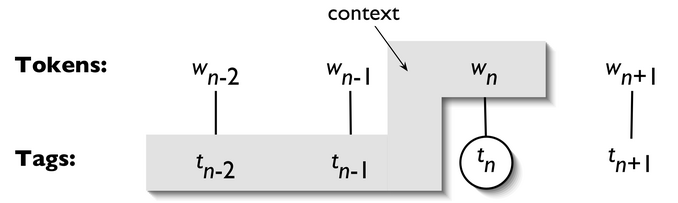
\includegraphics[width=0.4\textwidth]{tag-context.png} 
\end{center}
\caption{Tagger Context}
\label{fig:trigram}
\end{figure}

The tag to be chosen, $t_{n}$, is circled, and the context is shaded in grey.
In the example of an n-gram tagger shown in figure \ref{fig:trigram}, we have $n=3$; that is, we consider the tags of the two preceding words in addition to the current word.
An n-gram tagger picks the tag that is most likely in the given context.
\par
Altrough we use the name trigram all throughtout this paper, we acctually refer to sequential tagger, which consists of
\textit{affix}\footnote{The Affix tagger learns prefix and suffix patterns to determine the part of speech tag for word.}, \textit{unigram}, \textit{bigram} and \textit{trigram} taggers in this order respectively. First we build affix, which is used as ad \textit{backoff-tagger} for unigram. Unigram is afterwards used as a backoff-tagger for bigram, which is finally used for trigram.

\subsection{Brill tagger} %BANIČ

The Brill tagger is another part-of-speech tagger and was first described by Eric Brill in 1993. Before trying to explain it, we must address issues with n-gram taggers (e.g. \textit{Trigram tagger}).

First issue with n-gram taggers is size of their n-gram table. If we want to use tagging process on mobile computing device, compromise must be taken between performance and model size. 

A second issue with n-gram tagger is, that the only information it considers from prior context is tags. This is not practical because words themselves are useful information also. Therefore n-gram taggers are impractical models to be used to identify words in context. 
  
To bypass those issues we can use \textit{Brill tagger}. It can be summarised as an transformation-based learning and performs very well using models that are just a fraction of the size of n-gram taggers.

Despite obvious differences between Brill tagger and n-gram tagger there is one similarity. Both of them use \textit{supervised learning} method, since we require annotated training data to make sure whether the tagger's guess is a mistake or not.

The idea behind the Brill tagger is: \textit{guess the tag of each word, then go back and fix the mistakes}. Basically, Brill tagger can transform bad tagging into a better one. 

\subsection[Naive Bayes classifier]{Naive Bayes classifier\footnote{Definition and images summerized from \cite{NLTKBOOK}}}
Both Brill and Trigram are sequential backoff taggers. Meanwhile, Naive Bayes is \textit{classifier based tagger}.
Classification is a process where, for a given output, we have to choose the correct class. Basically, it is an  procedure for assigning  input data into one of a given number of categories.

Examples of classification tasks are:
\begin{itemize}
\item whether an email is spam or not.
\item diagnosis to a given patient as described by observed characteristics of the patient
\end{itemize}
The basic classification task has a number of interesting variants. For example, in multi-class classification, each instance may be assigned multiple labels; in open-class classification, the set of labels is not defined in advance; and in sequence classification, a list of inputs are jointly classified.

Every feature in naive Bayes classifier can determine which label can be assigned to a given input. Choosing a label for an input is a process, that consists of calculating the prior probability of each label (it is determined by calculating frequency in training set). Priori probability is combined with contribution from each feature. This is necessary to get the likelihood estimate for each label. Input value is then assigned the label whose likelihood estimate is the highest. The process is shown in \ref{fig:naive-bayes-triangle}.

\begin{figure}[htb]
\begin{center}
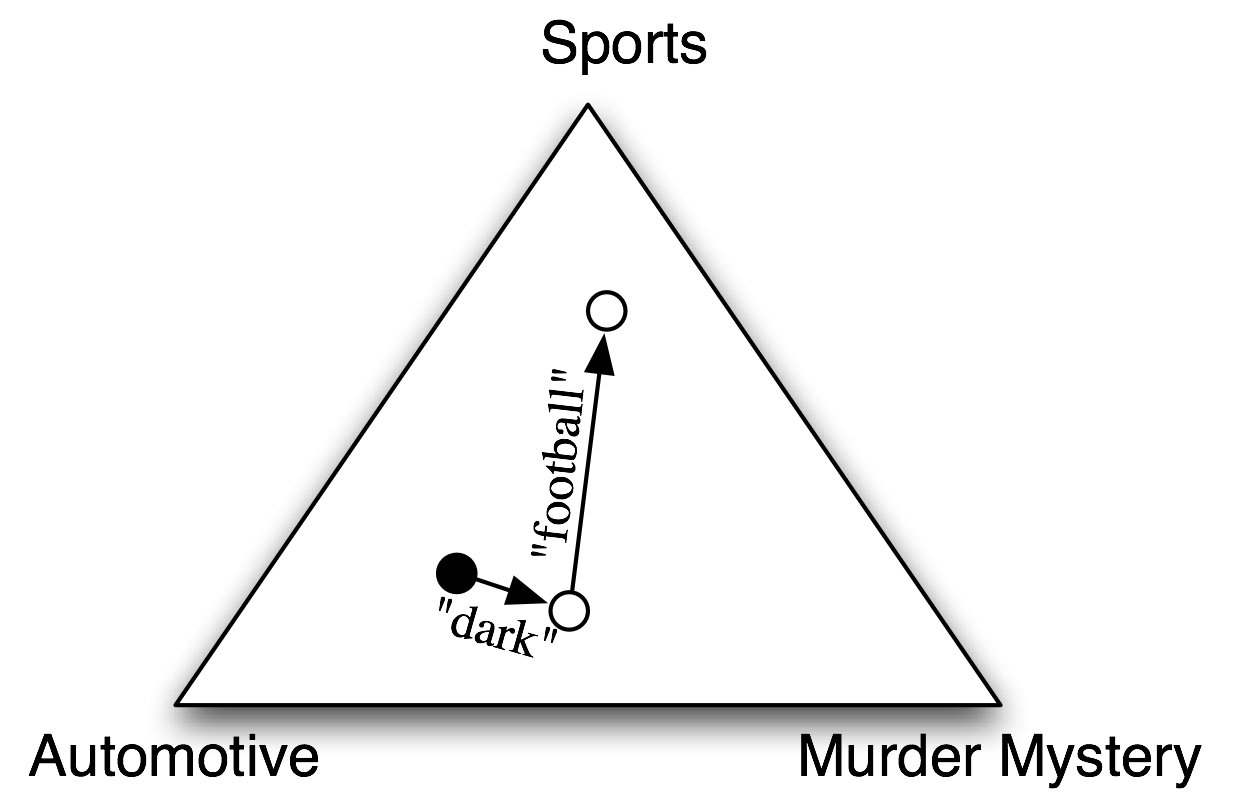
\includegraphics[width=0.4\textwidth]{naive-bayes-triangle.png} 
\end{center}
\caption{An illustration of the procedure used by the naive Bayes classifier to choose the topic for a document.}
\label{fig:naive-bayes-triangle}
\end{figure}

Let's assume that in the training corpus most documents have automotive topic. Because of this assumption, the classifier starts near "automotive" label. Later it must take into consideration the effect of each feature. Example considers, that input document contains word "dark", which indicates for "murder mystery", but also contains the word "football", which (strongly) indicate for "sports". After every feature has made its contribution, the classifier checks which label it is closest to, and assigns that label to the input.

Features make their contribution to the  decision by voting against those labels, that don't occur with this feature. Likelihood score is therefore reduced for each label by multiplying it with the probability that an input value with that label would have that feature. Suppose that the word occurs ran occurs in  12\% of the sports documents, 10\% of the murder mystery documents, and 2\% of the automotive documents. The likelihood score for the sports label will be multiplied by 0.12, the likelihood score for the murder mystery label will be multiplied by 0.1, and the likelihood score for the automotive label will be multiplied by 0.02. The overall effect will be to slightly reduce the score of the sports label, reduce the murder mystery label (more then sports label) and significantly reduce the automotive label. Figure \ref{fig:naive-bayes-bargraph} illustrates this example.

\begin{figure}[htb]
\begin{center}
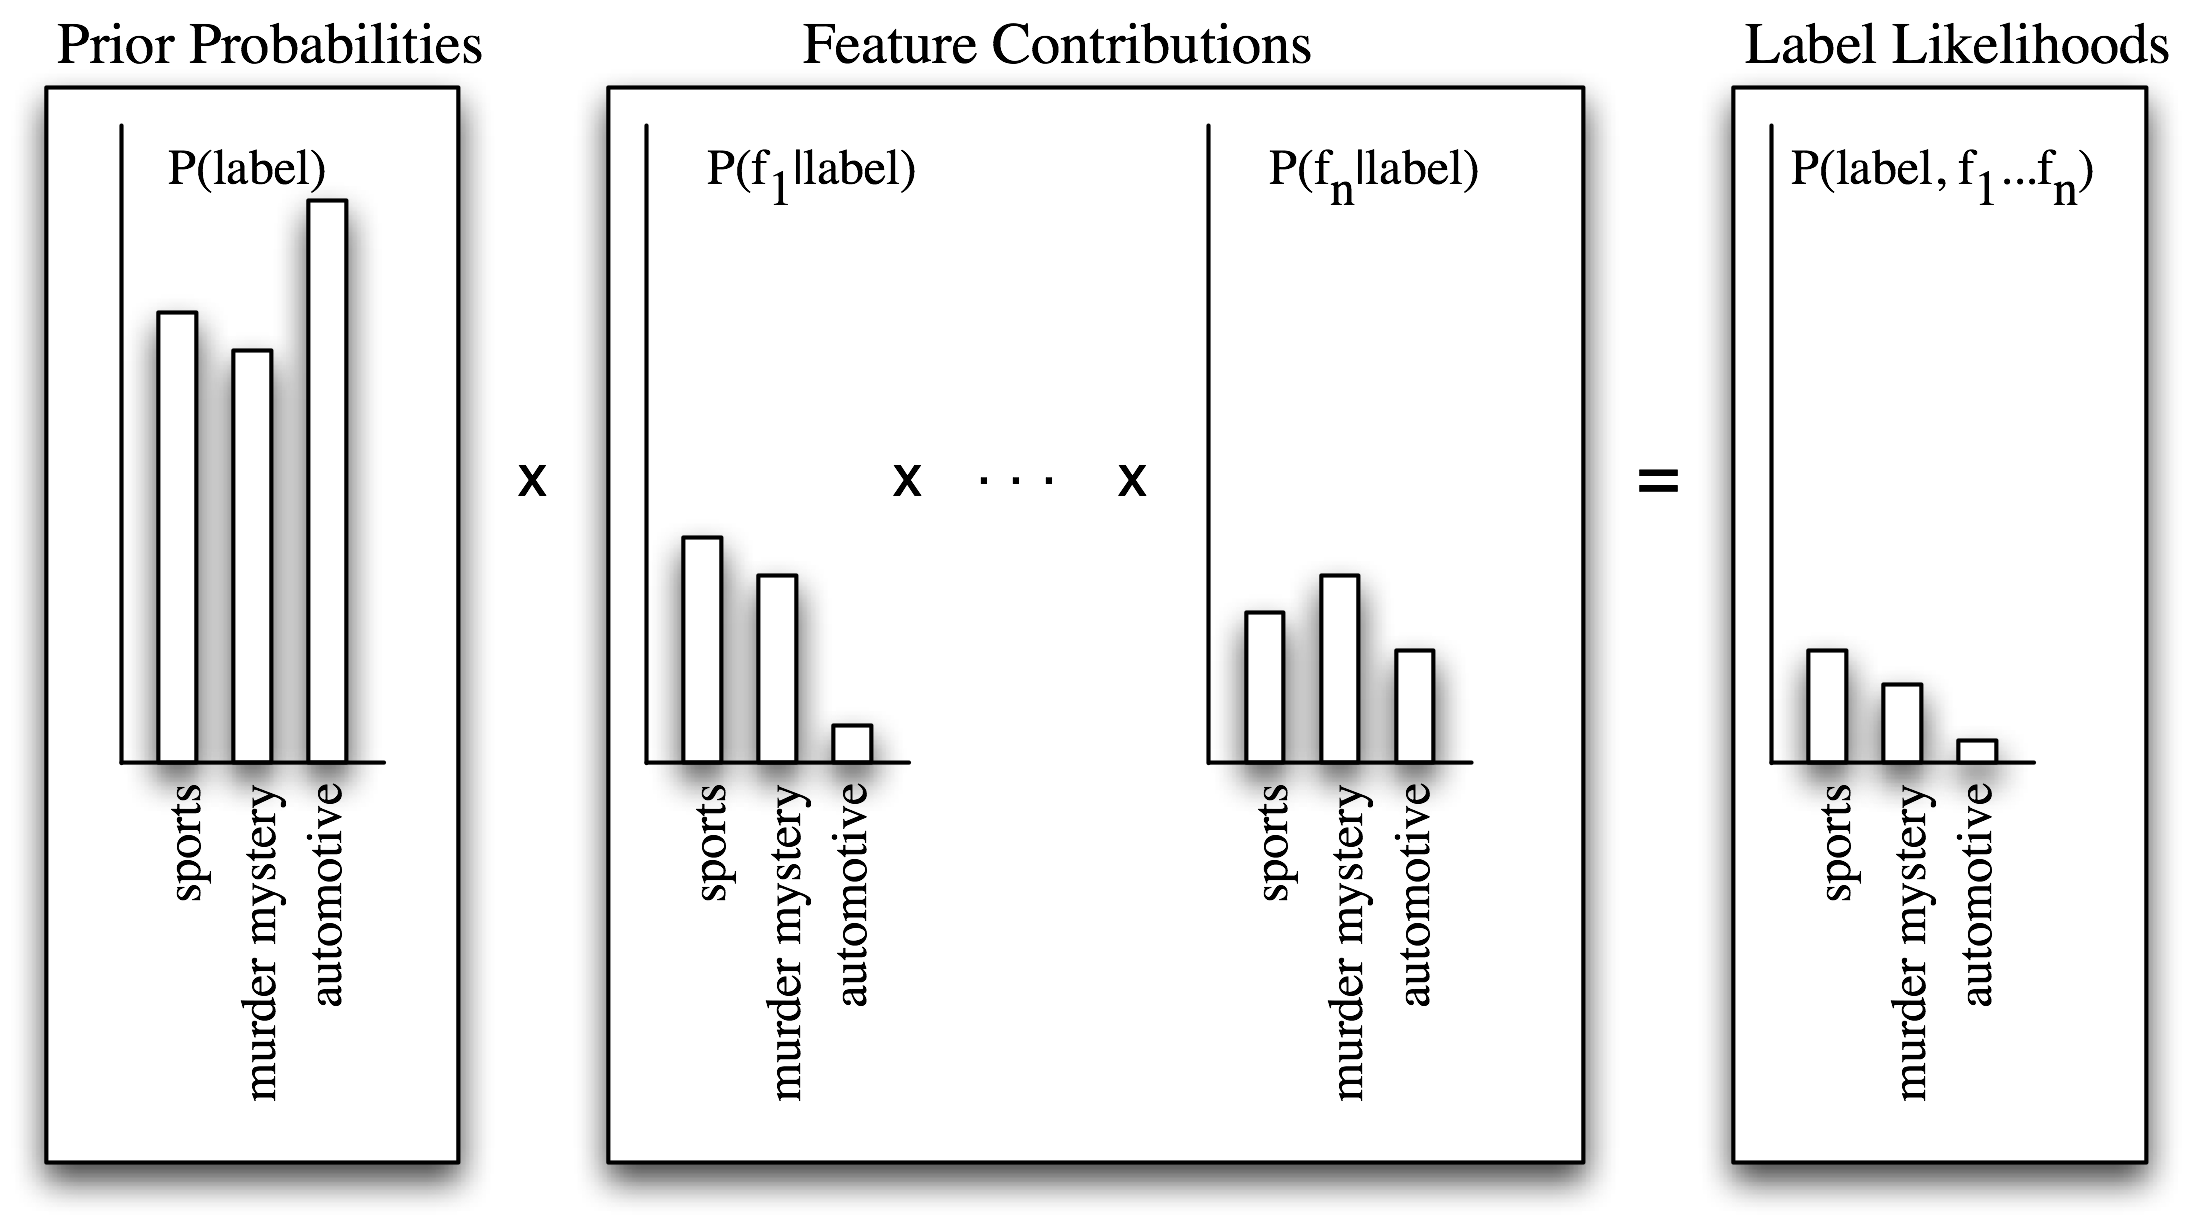
\includegraphics[width=0.4\textwidth]{naive_bayes_bargraph.png} 
\end{center}
\caption{Illustrating the process of calculating label likelihoods with naive Bayes.}
\label{fig:naive-bayes-bargraph}
\end{figure}

\section{Related work}
\label{relatedWork}
\subsection{Nltk-trainer} %NIKICC
The code for building the tagger was taken from \textit{Nltk-trainer}  project \cite{nltk-trainer}, whose author is Jacob Perkins.
Its an open-source project hosting on Github, with moto to \textit{Train NLTK objects with zero code}.
We almost exclusively used the script \texttt{train\_tagger.py}, which has the ability to generate NLTK taggers. This project made it a lot easier for us to train the taggers on Slovenian corpuses.

\subsection{JOS corpus} %BANIČ
The basic component for building Slovene tagger is \textit{JOS corpus} from JOS project \cite{JOS}. It stands for: \textit{Jezikoslovno Označevanje Slovenskega jezika} (Linguistic annotation of Slovenian language).
It contains collections of various text in Slovenian language with annotation.
For our project we used jos1M corpus that contain 1 million words with it's appropriate lemmas and morphosyntactic descriptions.
The JOS is compatible with Slovene\textit{ MULTEXT-East morphosyntactic specifications Version 4}\cite{MULTEXT-East}.
It basic purpose is to define word classes.
For each class there are various attributes and their appropriate values, which they can be mapped into morphosyntactic descriptions (i.e. MSD).
The structure of JOS corpora is in  \textit{Extensible Markup Language (XML)}.

\section{Implementation}
\label{implementation}
\subsection{Corpus transformation} %BANIČ
\label{Corpus transformation} 

We can easily manipulate XML files in various programming languages (e.g. Python with xml.dom.minidom).
This is mandatory because \textit{nltk-trainer}\cite{nltk-trainer} expects special form of input file (.pos file).

The first step for corpus transformation is to identify proper \textit{XML tags}\cite{xml_tags} in JOS corpora. There are several types, but we must parse only those in \textit{sentence tag }(\textit{<s>}):
\begin{itemize}
\item \textit{<S>} - space.
\item \textit{<c>} - character i.e. punctuation marks (e.g. period (.), comma (,), colon (:), ... ).
\item \textit{<w>} - word.
\item \textit{<term>} - a word or group of words designating something, especially in a particular field. 
\end{itemize}

For nltk-trainer to work, we must transform \texttt{jos1m.xml} to \texttt{.pos} file, which contains words with their morphosyntactic descriptions and punctuation marks. The correct syntax is shown in the next example:
\begin{lstlisting}
Britanski/Ppnmeid BBC/Slmei ,/,  brez/Dr 
\end{lstlisting}

The trainer will train the tagger properly, if in .pos file:
\begin{itemize}
\item The words and their MSD are separated with slash.
\item Every punctuation mark is separated with slash and then follows the same punctuation mark.
\item Words and punctuation marks are between space.
\end{itemize}

If we follow these "rules", implementation is simple. We just need to go through all child tags in sentence tag and properly write them in a file. Because Slovenian language contain letters with caron, proper encoding of tags must be provided. This is simply done with function \textit{encode()} (e.g. encode("utf-8") - this is proper encoding for Slovenian language).
\textit{Jos1M} corpus is build up with 10 XML files (e.g. \texttt{jos1M-01.xml},  \texttt{jos1M-02.xml}, ..., \texttt{jos1M-10.xml}), so we must parse all of them. 
File \texttt{transformJOS.py} contains the corpus transformation.

\subsection{Training the tagger} %NIKICC
As mentioned above, the script \texttt{train\_tagger.py} was used for this purpose. Its mandatory argument is a corpus in .pos format, which generation is described in \ref{Corpus transformation}. Beside this, there are many optional arguments. Here we will describe basics, for further description run script help with
\begin{lstlisting}
train_tagger.py --help
\end{lstlisting}
\par
One is wheather to generate a Sequential Tagger, a Brill Tagger or a Classifier Based Tagger. For Sequential we can then select sequential backoff algorithm. This can be any combination of the following letters:
\begin{itemize}
\item a: AffixTagger
\item u: UnigramTagger
\item b: BigramTagger
\item t: TrigramTagger
\end{itemize}
The default is \textit{aubt}, which was used for our Trigram tagger, but you can set this to the empty string to not train a sequential backoff tagger. The Brill Tagger is trained in front of the other tagger, which in our implementation was the Trigram tagger. When building classifier based algorithm, we must select the classifier or the sequence of classifier. Following are supported: NaiveBayes, DecisionTree, Maxent, GIS, IIS, CG, BFGS, Powell, LBFGSB, Nelder-Mead, MEGAM and TADM. We should mention, that the time spent for training classifier based tagger, is much larger than, the time for a sequential or brill.
\par
Script also has the possibility to set default tag. We used \textit{-Neznan-}, which is Slovene word for \textit{-unknown-}.
\par
Last argument, that should be mentioned, is wheather to evaluate the tagger or not and the procentage of sentaces to be used. The default value is 1, which means that the \textit{same} sentances are first used for training the tagger and then for evaluation. We recommend this argument to be set below 1. If so, the right approach is used.
Sentances are devided into two groups, one in used for training and second for evaluation. \textit{Fraction} is the procentage of sentances assigned to training group. 
This was used for evaluating constructed taggers. For results of this evaluation see section \ref{results}).

\subsection{Usage with NLTK} %BANIČ

We can use the trained tagger and NLTK to see how they can be used in Slovenian language. The requirements are installed NLTK and Python 2.7. We set an example in file \texttt{example.py}.
First we need to import following functions:
\begin{itemize}
\item[•] \textit{pickle} - it is a module for serialization and de-serialization a Python object structure ("pickling" - Python object hierarchy is converted into a byte stream). Pickle is used for loading classifiers such as Trigram tagger, Brill tagger, etc.
\begin{lstlisting}
tagger = pickle.load( open("slovene_taggers/BrillTagger.pickle") )
\end{lstlisting}

\item[•] \textit{PunktWordTokenizer} \cite{tokenizer} - it  is just one of many NLTK's tokenizers, that can be used to divide strings into lists of substring. Tokenizers are subclasses of \textit{nltk.tokenizer.TokenizerI} interface, which defines the \textit{tokenizer()} method. PunktWordTokenizer uses regular expressions to divide a word into tokens. These tokens are then used by the tagger. Following example will demonstrate, how does PunktWordTokenizer tokenize a sentence. If we have the following sentence:

\textit{Potem se je obrnil proti nam in skozi solze izoblikoval najlepši nasmeh, kar sem jih videl v življenju.}\\
the tokenizer will output the following list of tokens:

[\textit{'Potem', 'se', 'je', 'obrnil', 'proti', 'nam', 'in', 'skozi', 'solze', 'izoblikoval', 'najlepši', 'nasmeh', ',', 'kar', 'sem', 'jih', 'videl', 'v', 'življenju.'}]

As you can see, there is the problem with the last dot. The solution we used is described below.

\item[•] \textit{nltk.data} - it is a module that contains various functions to load NLTK files, such as corpora. We use it for \textit{sentence segmentation}. In some cases user can input not a sentence, but a whole paragraph. Before using PunktWordTokenizer to tokenize sentence into tokens, we need to segment it into sentences. This can be easily used by including Slovene Punkt sentence segmenter. Following example shows, how does sentence segmenter work. If we have the following paragraph:

\textit{Zdravljíca je pesem, ki jo je France Prešeren napisal novembra leta 1844. Po 6. členu ustave je Zdravljica besedilo himne Republike Slovenije. Melodija je iz istoimenske zborovske skladbe skladatelja Stanka Premrla.}\\

the sentence segmenter will output the following list of sentences:

[\textit{'Zdravljíca je pesem, ki jo je France Prešeren napisal novembra leta 1844.', 'Po 6. členu ustave je Zdravljica besedilo himne Republike Slovenije.', 'Melodija je iz istoimenske zborovske skladbe skladatelja Stanka Premrla.'}]
\end{itemize} 


The first step is to use sentence segmenter, to form a list of sentences. This list is then being tokenized with PunktWordTokenizer. One drawback with this tokenizer is that it doesn't tokenize the last word of a sentence and the following period (as shown in the example). Before using the PunktWordTokenizer, we must divide them with space. After we tokenize the sentences, tagging can be used. The result is a list of tuples with words or characters and their appropriate morphosyntactic description. 

We also implemented a function that returns two description dictionaries for MSDs with attribute=value expansions in Slovene and English. This way user can view which part-of-speech words belong to in Slovene or English. Following example demonstrates the expected output:
\\\\
\textit{( Lep  |  PPNMEIN ) - pridevnik \\
	( je  |  GP-STE-N ) - glagol\\
	( dan  |  SOMEI ) - samostalnik\\
	( ,  |  , ) - ni razlage\\
	( vse  |  ZC-SEI ) - zaimek\\
	( diši  |  GGNSTE ) - glagol\\
	( že  |  L ) - členek\\
	( po  |  DM ) - predlog\\
	( pomladi  |  SOZEM ) - samostalnik\\
	( !  |  ! ) - ni razlage}\\

We must exmplain, that here only the part of whole MSD is printed. For example the whole MSD for \textit{Lep} shown in table \ref{tab:MSDLep}.

\begin{table}[h]
\begin{center}
\begin{tabular}{c|c}
\multicolumn{2}{c}{pridevnik}\\\hline\hline
vrsta & splošni \\
spol & moški \\
število & ednina \\
sklon & imenovalnik \\
živost & 0 \\
vid & 0 \\
oblika & 0 \\
oseba & 0 \\
nikalnost & 0 \\
stopnja & nedoločeno \\
določnost & ne \\
število\_svojine & 0 \\
spol\_svojine & 0 \\
naslonskost & 0 \\
zapis & 0 \\
\end{tabular}
\end{center}
\caption{Whole MSD for \textit{Lep} in Slovene}
\label{tab:MSDLep}
\end{table}

The first output was creted with function \textit{prettyPrintWithDescription}, full output can be created with \textit{prettyPrintWithFullDescription}. Both function are defined in \texttt{example.py}
\par
But there is an issue. Because Slovenian language contain letters with caron, the output will have unicode symbols for them. In the previous examples, the output is already corrected. Solution is described in the following section. 

\subsection{Encoding problems} %BANIČ
Printing the result of our example is not optimal. Because we want users to know what these characters are, we implemented a solution. To resolve this, we must decode every word to \textit{UTF - 8} (because words we tag are in UTF - 8). If a user wants to print the result in "pretty" form, he should call function \textit{prettyPrint()} or \textit{prettyPrintByLine()} (both are implemented in \texttt{example.py}).

\section{Results} %NIKICC
\label{results}
For all constructed taggers, we here provide their accuracy. The results were obtained by repeating the proces of building the tagger with various evaluation arguments (see script \texttt{evaluateTaggers.sh}). See table \ref{tab:evaluation} and figure \ref{fig:evaluation}.

\begin{table}[h]
\begin{center}
\begin{tabular}{c|c|c|c}
\textit{fraction} & \textit{Trigram} & \textit{NaiveBayes} & \textit{Brill} \\\hline\hline
0.75  &  0.8286  &  0.8451  &  0.8490\\
0.80  &  0.8304  &  0.8461  &  0.8514\\
0.82  &  0.8306  &  0.8465  &  0.8515\\
0.84  &  0.8299  &  0.8462  &  0.8508\\
0.86  &  0.8306  &  0.8472  &  0.8512\\
0.88  &  0.8299  &  0.8474  &  0.8517\\
0.90  &  0.8288  &  0.8467  &  0.8507\\
0.91  &  0.8278  &  0.8462  &  0.8489\\
0.92  &  0.8276  &  0.8464  &  0.8490\\
0.93  &  0.8281  &  0.8464  &  0.8491\\
0.94  &  0.8278  &  0.8461  &  0.8496\\
0.95  &  0.8289  &  0.8475  &  0.8510\\
0.96  &  0.8388  &  0.8538  &  0.8609\\
0.97  &  0.8401  &  0.8568  &  0.8612\\
0.98  &  0.8417  &  0.8588  &  0.8629\\
0.99  &  0.8379  &  0.8567  &  0.8578\\\hline\hline
\textit{average} & \textbf{0.8317} & \textbf{0.8490} & \textbf{0.8529}
\end{tabular}
\end{center}
\caption{Taggers accuracy for various fractions.}
\label{tab:evaluation}
\end{table}

\begin{figure}[h]
\begin{center}
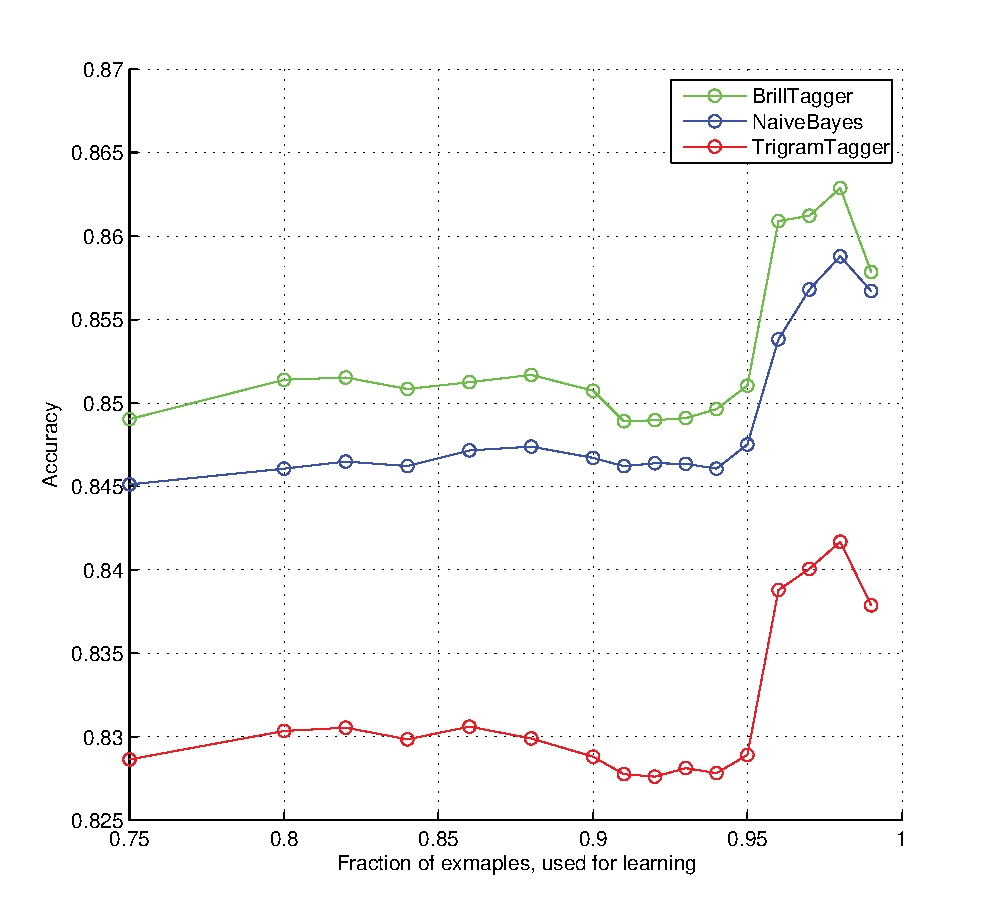
\includegraphics[width=0.5\textwidth]{../evaluation/graph.pdf} 
\end{center}
\caption{Accuracy evaluation results.}
\label{fig:evaluation}
\end{figure}
\par
To conclude, there are no major differences in tagging accuracy. The Brill and the Naive Bayes are about 2\% better than Trigram.
\par
However, during this evaluation we discover an other parameter, which should be taken into account.
Under the assumption that most of the time was actually spent for tagging the sentences (besides just testing for equality and percentage calculation are needed), we noticed that the time for evaluations differ drastically.
The results of resarching time consumption are listed in table \ref{tab:evaluation_speed} and graphically represented on figure \ref{fig:evaluation_speed} (see script \texttt{evaluateTaggersSpeed.py}).

\begin{table}[h]
\begin{center}
\begin{tabular}{c|c|c|c}
\textit{number of words} & \textit{Trigram} & \textit{NaiveBayes} & \textit{Brill} \\\hline\hline
   50  &  0.0003 &   4.1543  &  0.0011\\
   75  &  0.0004 &   6.2464  &  0.0014\\
  100  &  0.0006 &   8.5232  &  0.0018\\
  125  &  0.0008 &  10.6370  &  0.0020\\
  150  &  0.0009 &  12.4937  &  0.0024\\
  175  &  0.0011 &  14.5484  &  0.0027\\
  200  &  0.0011 &  16.3944  &  0.0029\\
  225  &  0.0013 &  18.6332  &  0.0032\\
  250  &  0.0015 &  20.7357  &  0.0035\\
  275  &  0.0017 &  22.8280  &  0.0041\\
  300  &  0.0018 &  24.8243  &  0.0042\\
  325  &  0.0018 &  27.4270  &  0.0043\\
  350  &  0.0022 &  29.2458  &  0.0051\\
  400  &  0.0023 &  32.9599  &  0.0052\\
  425  &  0.0024 &  36.0322  &  0.0056\\
  450  &  0.0027 &  38.1471  &  0.0062\\
  475  &  0.0027 &  39.2278  &  0.0064\\
  500  &  0.0029 &  41.2688  &  0.0063\\
\end{tabular}
\end{center}
\caption{Time spent in seconds for tagging different numbers of words.}
\label{tab:evaluation_speed}
\end{table}

\begin{figure}[h]
\begin{center}
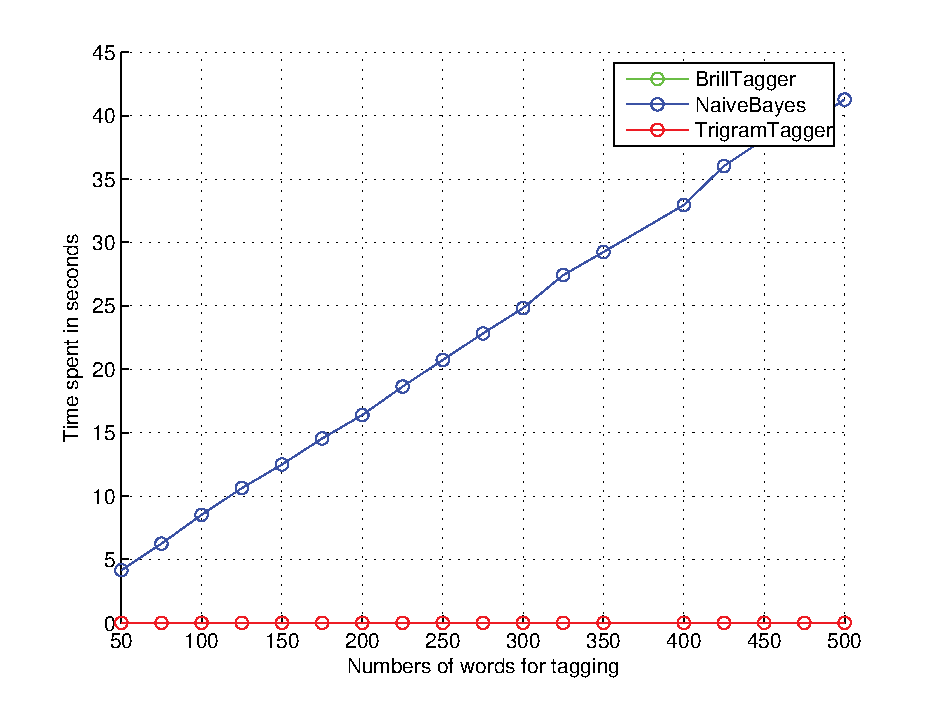
\includegraphics[width=0.5\textwidth]{../evaluation/graph_speed.pdf} 
\end{center}
\caption{Spent time measurements. NOTE: The green line is not visible because it is right under the red one.}
\label{fig:evaluation_speed}
\end{figure}

The difference here is enormous. Brill and Trigram run at almost the same speed, while Naive Bayes runs extremely slower. This is also one of the reason why we prefer usig the Brill tagger. 

\section{Conclusion} %BANIČ
To conclude our paper, tagging in Slovene language is practical with proper use of Natural Language Toolkit and \textit{nltk-trainer}. Time spent in seconds for tagging different numbers of words, show that Brill and Trigram ran at the same speed, while Naive Bayes ran drasticly slower. There are no major differences in tagging accuracy. However Brill and the Naive Bayes are about 2\% better than Trigram.
\par
Besides these three taggers we built, others can be built without any bigger modification. All that is needed is to set some arguments when calling the script \texttt{train\_tagger.py}. The main reason we built only these three is computing power. These three are the only one we could built and evaluate in some resonable time.
\par
Our whole project is publicly available on github \cite{CODE}. We also contacted the NLTK developers group and will arrange our taggers to become the part of NLTK.

\section*{Acknowledgements}
We would like to express our gratitude to all the contributors of \textit{JOS} \cite{JOS} project, \textit{nltk-trainer} \cite{nltk-trainer} project and to Marko Robnik-Šikonja, PhD, Associate Professor, who was our mentor at Faculty of Computer and Information Science. Also this project would not be possible without \textit{Natural Language Toolkit} \cite{nltk} and their admirable documentation.

\begin{thebibliography}{99}
\bibitem{nltk} \url{http://www.nltk.org/}
\bibitem{JOS} \url{http://nl.ijs.si/jos/}
\bibitem{nltk-trainer} \url{https://github.com/japerk/nltk-trainer}
\bibitem{MULTEXT-East} \url{http://nl.ijs.si/ME/V4/msd/html/msd-sl.html}
\bibitem{NLTKBOOK} \url{http://www.nltk.org/book}
\bibitem{xml_tags} \url{http://nl.ijs.si/ssj/schema/tei_ssj_doc.pdf}
\bibitem{tokenizer} \url{http://docs.huihoo.com/nltk/0.9.5/guides/tokenize.html}
\bibitem{CODE} \url{https://github.com/nikicc/slovene-nltk-tagger}
\end{thebibliography}
\end{document}